\section{The reduction to abelian varieties}\label{sec:reduction}

\subsection{The statement \Fiii{} and the class $\mathcal{A}$}

\begin{definition}\label{def:f3prime}
For a variety $X$ and $p\ge0$ let $\Ab^{p}(X)\subseteq H^{2p}(X)$ be the span of the classes $\Gamma_{*}\gamma$ of degree $2p$, where $B$ runs over the complex abelian varieties, the point included, $\gamma$ over $\Hdg^{*}(B)$, and $\Gamma$ over the algebraic cycles on $B\times X$ with rational coefficients. The statement \Fiii{} is: $\Hdg^{p}(X)=\Ab^{p}(X)$ for every $X$ and every $p$.
\end{definition}

Each $\Gamma_{*}\gamma$ is a Hodge class, since cup product with an algebraic class and push-forward along a projection are morphisms of Hodge structures of the right bidegree; so $\Ab^{p}(X)\subseteq\Hdg^{p}(X)$. Taking $B$ a point shows that $\Ab^{p}(X)$ contains every algebraic class, and taking $X$ abelian, $B=X$ and $\Gamma$ the diagonal shows that \Fiii{} holds on every abelian variety.

\begin{proposition}\label{prop:hc-split}
$\HC$ holds if and only if $\AB$ and \Fiii{} both hold.
\end{proposition}

\begin{proof}
If $\HC$ holds then $\AB$ holds, and every Hodge class is algebraic, hence in $\Ab^{p}(X)$. Conversely let $\gamma\in\Hdg^{p}(X)$. By \Fiii{}, $\gamma=\sum_{j}\Gamma_{j*}\gamma_{j}$ with $\gamma_{j}$ a Hodge class on an abelian variety $B_{j}$, algebraic by $\AB$; then $\mathrm{pr}_{B_{j}}^{*}\gamma_{j}\cup[\Gamma_{j}]$ is algebraic on $B_{j}\times X$ and so is its push-forward to $X$.
\end{proof}

\begin{proposition}\label{prop:f3prime-known}
Let $\mathcal{A}$ be the class of varieties $X$ such that $H^{*}(X)$ is spanned by classes $\Gamma_{*}y$ with $B$ abelian, $\Gamma$ an algebraic cycle on $B\times X$ and $y\in H^{*}(B)$.
\begin{enumerate}[label=\textup{(\roman*)},leftmargin=2.4em,itemsep=2pt]
\item Every $X\in\mathcal{A}$ satisfies \Fiii{}.
\item $\mathcal{A}$ contains the abelian varieties and the curves, and is closed under products and under images of surjective morphisms. It contains every product of curves, every symmetric product of a curve, and every variety dominated by a product of curves or by an abelian variety.
\item Every $X$ of dimension $d$ satisfies \Fiii{} in the degrees $2p$ with $p\in\{0,1,d-1,d\}$. In particular every variety of dimension at most three satisfies it in every degree.
\end{enumerate}
\end{proposition}

\begin{proof}
(i) Let $\gamma\in\Hdg^{p}(X)$ and write $\gamma=\sum_{j}\Gamma_{j*}y_{j}$ with $y_{j}\in H^{*}(B_{j})$. Each $\Gamma_{j*}$ is a morphism of Hodge structures, so after replacing $y_{j}$ by its component in the degree that $\Gamma_{j*}$ sends to $2p$ we may assume $y_{j}$ homogeneous. Let $\pi_{j}$ be the projector of $H^{*}(B_{j})$ onto its Hodge classes along a complement stable under the Hodge group, which exists because that group is reductive. Then $\gamma=\sum_{j}\Gamma_{j*}\pi_{j}y_{j}+\sum_{j}\Gamma_{j*}(1-\pi_{j})y_{j}$. The second sum is a Hodge class whose summands lie in images of Hodge complements of the invariants; the Hodge group of $\prod_{j}B_{j}\times X$ acts on each term through a representation without invariants, so each term, being a Hodge class, is zero. Hence $\gamma=\sum_{j}\Gamma_{j*}(\pi_{j}y_{j})\in\Ab^{p}(X)$.

(ii) The point, abelian varieties and curves are in $\mathcal{A}$: for a curve $C$, $H^{0}$ and $H^{2}$ come from the point and $H^{1}(C)=H^{1}(J(C))$ by the Abel--Jacobi map. If $X,Y\in\mathcal{A}$ then $H^{*}(X\times Y)=H^{*}(X)\otimes H^{*}(Y)$ is spanned by exterior products of classes $\Gamma_{*}y\boxtimes\Gamma'_{*}y'=(\Gamma\times\Gamma')_{*}(y\boxtimes y')$ with $B\times B'$ abelian. If $f\colon X\to X'$ is surjective, then $f_{*}f^{*}=\deg(f)$ on $H^{*}(X')$ after cutting $X$ by hyperplanes to the dimension of $X'$ if needed, so every class of $X'$ is $f_{*}$ of a class of $X$, and $f_{*}\Gamma_{*}y=(\Gamma_{f}\circ\Gamma)_{*}y$ with $\Gamma_{f}$ the graph of $f$. The listed varieties follow: a symmetric product is the image of a product of curves, and a variety dominated by a product of curves or an abelian variety is such an image.

(iii) Degrees $0$ and $2d$ are spanned by the class of $X$ and the class of a point. In degree $2$ every Hodge class is a divisor class by Lefschetz \cite{Lef24}. In degree $2d-2$, let $\theta$ be a hyperplane class; the hard Lefschetz theorem makes $\theta^{d-2}\cup\colon H^{2}(X)\to H^{2d-2}(X)$ an isomorphism of Hodge structures, so every Hodge class of degree $2d-2$ is $\theta^{d-2}\cup\alpha$ with $\alpha$ a Hodge class of degree $2$, algebraic by Lefschetz; a product of algebraic classes is algebraic.
\end{proof}

\subsection{The statement \Fii{}}

For an abelian variety $Y$ let $R(Y)\subseteq H^{*}(Y)$ be the $\QQ$-subalgebra generated by the divisor classes of $Y$ and by the pull-backs $f^{*}w$ of Weil classes $w$ of abelian varieties $B$ of Weil type along homomorphisms $f\colon Y\to B$. Every element of $R(Y)$ is a Hodge class, and every Hodge class on an abelian variety of dimension at most five lies in $R(Y)$ \cite{MZ99}.

\begin{definition}\label{def:f2}
The statement \Fii{} is: for every complex abelian variety $Y$, every Hodge class on $Y$ that does not lie in $R(Y)$ is algebraic.
\end{definition}

The classes in $R(Y)$ are the ones the known theorems reach when they reach anything: divisor classes by Lefschetz, Weil classes by Markman \cite{Mar25a,Mar25b,Mar25c} on fourfolds of Weil type and by the propagation results of \cite{BMB26} wherever they propagate. So \Fii{} is the conjecture for abelian varieties with the known classes struck out. The next proposition says that striking them out removes nothing.

\begin{setup}\label{setup:mumford}
Let $X$ be a Mumford fourfold, $V=H^{1}(X)$ with its polarisation $\psi$, $G=\Hg(X)\subseteq\Sp(V,\psi)$, and $e_{0}\in\Hdg^{2}(X\times X)$ an exceptional class, a Hodge class of degree four that is not a polynomial in divisor classes. Such classes exist \cite{MZ95};\footnote{Mumford constructed \cite{Mum69} abelian fourfolds $X$ whose Hodge group is a $\QQ$-form of $\mathrm{SL}_{2}^{3}$ acting on $H^{1}(X)$, of dimension eight, through the tensor product of the three two-dimensional representations; the form comes from a quaternion algebra over a totally real cubic field $F$ that is split at one real place and ramified at the other two, and the corestriction to $\QQ$ of that algebra is the matrix algebra, which is what makes the representation rational. Such an $X$ is simple, has $\End^{0}(X)=\QQ$, is not of CM type, and its Hodge group is smaller than the full symplectic group although no endomorphism accounts for the loss; its Shimura curve is compact. The exceptional classes of \cite{MZ95} live in degree four on $X\times X$ (equivalently in $\End$ of $H^{1}$ as a Hodge structure of weight zero) and span the invariants of the Hodge group that are not generated by the polarisation, and no one has proved them algebraic. The fourfold enters this paper because it is the smallest variety on which \Fii{} has an unsettled instance that no CM point reaches directly.} $X$ is simple with $\End^{0}(X)=\QQ$ \cite{Mum69}.
\end{setup}

\begin{lemma}\label{lem:sp-invariance}
Let $Y$ be an abelian variety. Let $Y_{X}\subseteq Y$ be the largest abelian subvariety isogenous to a power of $X$ and $Y'$ the identity component of the intersection of the kernels of the homomorphisms $Y\to X$. Then $Y_{X}\times Y'\to Y$ is an isogeny, $\Hom(X,Y')=0$, and
\[
H^{1}(Y)=\bigl(V\otimes Q\bigr)\oplus H^{1}(Y'),\qquad Q=\Hom^{0}(Y_{X},X),
\]
the first summand embedded by $v\otimes f\mapsto f^{*}v$. Let $\Sp(V,\psi)$ act on $H^{*}(Y)=\bigwedge^{*}H^{1}(Y)$ through the factor $V$. Then every class of $R(Y)$ is invariant under $\Sp(V,\psi)$, and for $Y=X^{m}$ the invariants of $\Sp(V,\psi)$ in $H^{*}(X^{m})$ are polynomials in divisor classes.
\end{lemma}

\begin{proof}
Poincar\'e reducibility gives $Y\sim Y_{X}\times Y'$ with $Y_{X}\sim X^{k}$ and no factor $X$ in $Y'$; since $X$ is simple, $\Hom(X,Y')=\Hom(Y',X)=0$, and since $\End^{0}(X)=\QQ$, $Q$ has dimension $k$ and the displayed map is an isomorphism. A homomorphism $h\colon Y\to Z$ of abelian varieties decomposes up to isogeny as $h_{X}\times h'$, and $h^{*}$ acts on $H^{1}$ as $(1\otimes(f\mapsto f\circ h_{X}))\oplus h'^{*}$, which commutes with the action of $\mathrm{GL}(V)$ on the factor $V$. So pull-backs along homomorphisms, cup products and exterior products are $\mathrm{GL}(V)$-equivariant, and the classes invariant under $\Sp(V,\psi)$ form a subalgebra stable under pull-back. It remains to check the generators of $R(Y)$.

A divisor class on $Y$ has K\"unneth components in $\bigwedge^{2}(V\otimes Q)$, $(V\otimes Q)\otimes H^{1}(Y')$ and $\bigwedge^{2}H^{1}(Y')$, each a Hodge class. The middle one is a homomorphism from $Y'$ to the dual of $Y_{X}$, which is zero. The first is a Hodge class on $Y_{X}$, hence a $G$-invariant of $\bigwedge^{2}(V\otimes Q)=S^{2}V\otimes\bigwedge^{2}Q\oplus\bigwedge^{2}V\otimes S^{2}Q$. Since $G$ contains the Hodge group of a simple abelian fourfold whose only Hodge classes of degree two are the divisor classes, $(S^{2}V)^{G}=0$ and $(\bigwedge^{2}V)^{G}=\QQ\psi$; so the component lies in $\psi\otimes S^{2}Q$, which $\Sp(V,\psi)$ fixes. The third component is fixed because $\mathrm{GL}(V)$ acts trivially on $H^{1}(Y')$.

For a Weil class, let $B$ be of Weil type for $K$ and $f\colon Y\to B$. The field $K$ acts on $B\sim B_{X}\times B'$ through $\End^{0}(B_{X})\times\End^{0}(B')$, because $\Hom(B_{X},B')=0$; so it acts on $Q_{B}=\Hom^{0}(B_{X},X)$ and on $H^{1}(B')$, and the eigenspace of $H^{1}(B,\bar\QQ)$ for an embedding $\sigma$ of $K$ is $V\otimes Q_{B,\sigma}\oplus H^{1}(B',\bar\QQ)_{\sigma}$. A Weil class lies in the sum over $\sigma$ of the top exterior powers of these eigenspaces, and $\bigwedge^{\mathrm{top}}(V\otimes Q_{B,\sigma}\oplus W_{\sigma})=(\det V)^{\otimes\dim Q_{B,\sigma}}\otimes(\det Q_{B,\sigma})^{\otimes 8}\otimes\det W_{\sigma}$, on which $\mathrm{SL}(V)\supseteq\Sp(V,\psi)$ acts trivially. Pulling back along $f$ preserves invariance.

For $Y=X^{m}$, $H^{*}(X^{m})=\bigwedge^{*}(V\otimes\QQ^{m})$, and the invariants of $\Sp(V,\psi)$ in the tensor algebra of $V$ are spanned by complete contractions with $\psi$ by the first fundamental theorem for the symplectic group \cite[Chap.~5]{GW09}; a contraction of two factors of $X^{m}$ is the pull-back of the class $\psi\in H^{2}(X\times X)$ along the projection to those factors, a divisor class, and a contraction within one factor is $\psi\in H^{2}(X)$. So the invariants are polynomials in divisor classes.
\end{proof}

\begin{theorem}\label{thm:f2isab}
\Fii{} implies $\AB$, and is therefore equivalent to it.
\end{theorem}

\begin{proof}
$\AB$ contains \Fii{}. Assume \Fii{}. By Lemma~\ref{lem:sp-invariance} the exceptional class $e_{0}$ is not invariant under $\Sp(V,\psi)$, since it is not a polynomial in divisor classes; as $\Sp(V,\psi)(\QQ)$ is Zariski dense in $\Sp(V,\psi)$, there is $g\in\Sp(V,\psi)(\QQ)$ with $ge_{0}\ne e_{0}$. Let $\theta$ be an ample class on $X\times X$, fixed by $g$ by the lemma.

Let $A$ be an abelian variety and $\beta\ne0$ a Hodge class of degree $2p$ on $A$, and put $Y=A\times X\times X$. The group $\Sp(V,\psi)$ acts on $H^{*}(Y)=H^{*}(A)\otimes H^{*}(X\times X)$ diagonally, through the copies of $V$ in both factors; on $H^{*}(A)$ it acts through $A_{X}$ and fixes $\beta$ when $\beta\in R(A)$, but we need only that $g(\beta\otimes e_{0})=g\beta\otimes ge_{0}$. If $\beta\otimes e_{0}$ lay in $R(Y)$ it would be fixed by $g$, so $g\beta\otimes ge_{0}=\beta\otimes e_{0}$, which forces $ge_{0}\in\QQ e_{0}$; and $g$ preserves the polarisation of $X\times X$, hence the intersection form on $H^{4}(X\times X)$ in which $e_{0}$ has nonzero square (the Hodge--Riemann relations on the primitive Hodge classes, after subtracting the part of $e_{0}$ in $\theta\cup H^{2}$, which is a polynomial in divisor classes and may be dropped from $e_{0}$ at the start), so $ge_{0}=\pm e_{0}$, and replacing $g$ by $g^{2}$ if needed, $ge_{0}=e_{0}$, a contradiction. So $\beta\otimes e_{0}\notin R(Y)$ and \Fii{} makes it algebraic. In the same way $e_{0}\cup\theta^{4}\notin R(X\times X)$: otherwise $(ge_{0}-e_{0})\cup\theta^{4}=0$, and $\theta^{4}\cup\colon H^{4}(X\times X)\to H^{12}(X\times X)$ is injective by hard Lefschetz. So \Fii{} makes every Hodge class of degree twelve on $X\times X$ algebraic.

The Hodge group of $X\times X$ is reductive, the Hodge classes of degrees four and twelve are its invariants, and Poincar\'e duality is an equivariant perfect pairing between $H^{4}$ and $H^{12}$; so it restricts to a perfect pairing between $\Hdg^{2}$ and $\Hdg^{6}$, and there is a Hodge class $e'$ of degree twelve with $\int_{X\times X}e_{0}\cup e'=1$. Then
\[
\beta=\mathrm{pr}_{A*}\bigl((\beta\otimes e_{0})\cup\mathrm{pr}_{X\times X}^{*}e'\bigr),
\]
a push-forward of a product of algebraic classes, is algebraic.
\end{proof}

Theorem~\ref{thm:intro-reduction} is Propositions~\ref{prop:hc-split}, \ref{prop:f3prime-known} and Theorem~\ref{thm:f2isab} together.

\subsection{The closure graph}\label{ssec:graph}

The paper \cite{BMB26} records the implications between the conjecture and the statements that have been used to approach it: the Lefschetz standard conjecture (L) for all varieties, the conjecture (M) that every Hodge class is motivated in Andr\'e's sense \cite{And96b}, the variational Hodge conjecture (V), the statement (F3) that the conjecture holds for all varieties that are not abelian, and the two statements of this paper.\footnote{For a smooth projective variety $X$ of dimension $d$ with hyperplane class $h$, (L) asks that the inverse of the hard Lefschetz isomorphism $h^{d-2p}\colon H^{2p}(X,\QQ)\to H^{2d-2p}(X,\QQ)$ be induced by an algebraic cycle on $X\times X$ for every $p$; it is known for abelian varieties, surfaces and the varieties whose cohomology is spanned by algebraic classes, and open for a general threefold. A Hodge class is motivated in Andr\'e's sense when it is obtained from classes of algebraic cycles by cup products, pull-backs, push-forwards and the inverse Lefschetz operators, on $X$ and on the products $X\times Y$; (M) asks that every Hodge class be of this kind, which is weaker than the conjecture by exactly the use of the inverse Lefschetz operator. (V) asks that a flat Hodge class in a smooth projective family be algebraic on every fibre once it is algebraic on one; Grothendieck observed that (V) follows from the conjecture, and the converse is open. (F3) concerns the varieties that are not abelian and makes no statement about abelian varieties at all; it is the complement, inside the conjecture, of \Fii{}, and the pair \Fii{}, (F3) is the coarsest division of the conjecture that this paper refines.} The rules are listed in Table~\ref{tab:rules}, each with the place where it is proved; the first two rows are Propositions~\ref{prop:hc-split} and Theorem~\ref{thm:f2isab}.

\begin{table}[t]
\centering
\caption{The rule set. A rule with two premises needs both. The closure of a set of statements under these rules, and the list of minimal sets whose closure contains $\HC$, are computed by hand in the text and checked in Lean (Appendix~\ref{app:checks}).}
\label{tab:rules}
\begin{ruledtabular}
\begin{tabular}{lll}
premises & conclusion & proof \\
\colrule
$\HC$ & (F3), \Fii{}, \Fiii{}, $\AB$, (M) & definitions; \cite{And96b} \\
(F3) & $\HC$ & \cite[Prop.~20.33]{BMB26} \\
\Fii{} & $\AB$ & Theorem~\ref{thm:f2isab} \\
$\AB$ & \Fii{} & definition \\
$\AB$, \Fiii{} & $\HC$ & Proposition~\ref{prop:hc-split} \\
(L), (M) & $\HC$ & \cite{And96b}; \cite[Thm.~20.70]{BMB26} \\
(L) & $\AB$ & \cite[Thm.~20.70]{BMB26} \\
(V) & $\AB$ & \cite[Thm.~20.70]{BMB26} \\
\end{tabular}
\end{ruledtabular}
\end{table}

\begin{proposition}\label{prop:minimal}
Under the rules of Table~\ref{tab:rules} the closure of a set of statements contains $\HC$ if and only if the set contains one of
\begin{widetext}
\begin{equation}\label{eq:minimal}
\{\mathrm{F3}\},\,\{\mathrm{L},\mathrm{M}\},\,\{\mathrm{L},\mathrm{F3}'\},\,\{\mathrm{V},\mathrm{F3}'\},\,\{\mathrm{F2},\mathrm{F3}'\},\,\{\AB,\mathrm{F3}'\},
\end{equation}
\end{widetext}
and these six sets are the minimal ones with this property.
\end{proposition}

\begin{proof}
Each listed set derives $\HC$: $\{\mathrm{F3}\}$ by the second row; $\{\mathrm{L},\mathrm{M}\}$ by the sixth; the other four through $\AB$, which \Fii{}, (L) and (V) each give, and the fifth row. For the converse, call a set closed if it is stable under the rules. A closed set without $\HC$ contains no (F3), does not contain (L) and (M) together, and, if it contains \Fiii{}, contains none of $\AB$, \Fii{}, (L), (V), since each of these yields $\AB$ and then $\HC$. The maximal closed sets without $\HC$ are therefore
\begin{align*}
M_{1}&=\{\mathrm{F2},\AB,\mathrm{L},\mathrm{V}\},\\
M_{2}&=\{\mathrm{F2},\AB,\mathrm{V},\mathrm{M}\},\\
M_{3}&=\{\mathrm{F3}',\mathrm{M}\},
\end{align*}
each of which is closed by inspection of the table. The closure of a set $\Sigma$ contains $\HC$ exactly when $\Sigma$ lies in none of the $M_{i}$. If $\Sigma$ contains (F3) this holds. Otherwise $\Sigma$ needs an element outside $M_{1}$, that is \Fiii{} or (M); one outside $M_{2}$, that is \Fiii{} or (L); and one outside $M_{3}$, that is one of \Fii{}, $\AB$, (L), (V). The minimal choices are \Fiii{} with one of \Fii{}, $\AB$, (L), (V), and (M) with (L). This gives the six sets, and each is minimal because removing any element lands in some $M_{i}$. The same computation is carried out mechanically from the rule list in the Lean file of Appendix~\ref{app:checks}, which returns these six sets and no others.
\end{proof}

Figure~\ref{fig:graph} draws the graph. The two statements of this paper are the nodes marked in colour; every route to $\HC$ other than (F3), which is $\HC$ itself, and (L)+(M) passes through \Fiii{}.

\begin{figure*}[t]
\centering
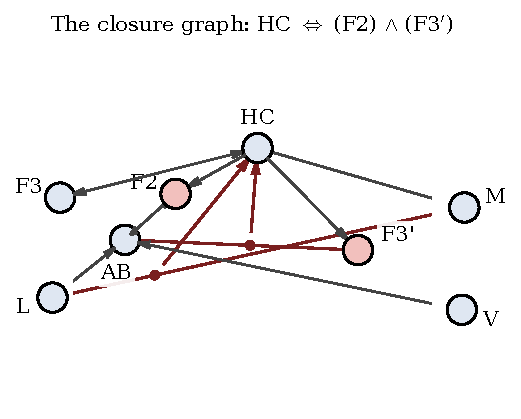
\includegraphics[width=0.92\textwidth]{figures/fig_graph}
\caption{The closure graph of Table~\ref{tab:rules}. Grey arrows are rules with one premise; a red fork joins the two premises of a rule that needs both. The coloured nodes are \Fii{} and \Fiii{}.}
\label{fig:graph}
\end{figure*}
